\documentclass{standalone}
\usepackage{tikz}
\usetikzlibrary{patterns}
\usetikzlibrary{positioning}
\usetikzlibrary{patterns, positioning}
\usetikzlibrary{shapes.misc}
\usepackage[outline]{contour}
\contourlength{1.5pt} 
\usetikzlibrary{calc}
        \usepackage{relsize}
        \tikzset{fontscale/.style = {font=\relsize{#1}}}

\begin{document}
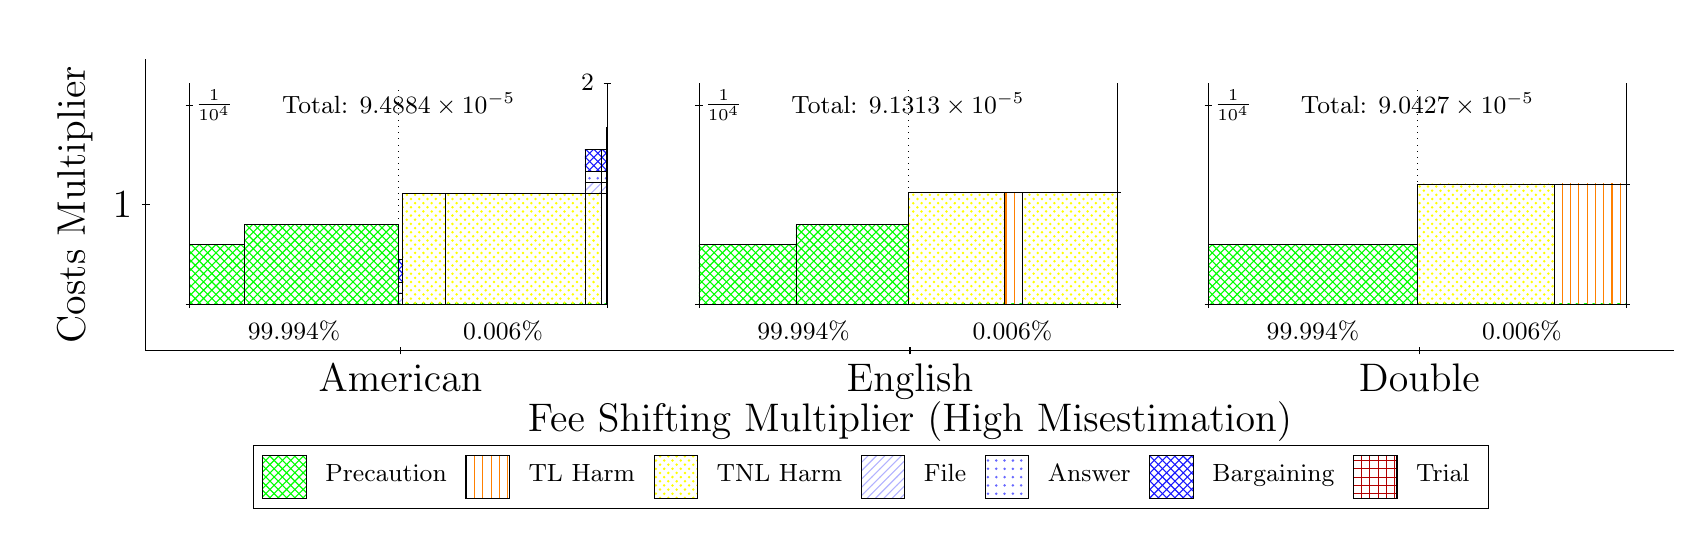
\begin{tikzpicture}
\clip(-0.5,-1.1) rectangle +(20.91,6.2);
\draw[black] (1,1) -- (1,4.7);
\node[rotate=90, fontscale=2, anchor=center] at (0.1, 2.85) {Costs Multiplier};
\draw[black] (0.95,2.85) -- (1.05,2.85);
\node[fontscale=2, anchor=east] at (0.95, 2.85) {1};

\draw[black] (1,1) -- (20.41,1);
\node[fontscale=2, anchor=center] at (10.705, 0.1) {Fee Shifting Multiplier (High Misestimation)};
\draw[black] (4.235,0.95) -- (4.235,1.05);
\node[fontscale=2, anchor=north] at (4.235, 0.95) {American};
\draw[black] (10.705,0.95) -- (10.705,1.05);
\node[fontscale=2, anchor=north] at (10.705, 0.95) {English};
\draw[black] (17.175,0.95) -- (17.175,1.05);
\node[fontscale=2, anchor=north] at (17.175, 0.95) {Double};


\draw[pattern=crosshatch, pattern color=green,draw=black,very thin] (1.5556,1.592) rectangle (2.2496,2.349);
\draw[pattern=crosshatch, pattern color=green,draw=black,very thin] (2.2496,1.592) rectangle (4.21,2.6014);
\draw[pattern=crosshatch, pattern color=green,draw=black,very thin] (4.21,1.592) rectangle (4.2553,1.592);
\draw[pattern=north east lines, pattern color=blue!30,draw=black,very thin] (4.21,1.592) rectangle (4.2553,1.7324);
\draw[pattern=dots,  pattern color=blue!60,draw=black,very thin] (4.21,1.7324) rectangle (4.2553,1.8728);
\draw[pattern=crosshatch,      pattern color=blue!90,draw=black,very thin] (4.21,1.8728) rectangle (4.2553,2.1536);
\draw[pattern=crosshatch, pattern color=green,draw=black,very thin] (4.2553,1.592) rectangle (4.2569,1.592);
\draw[pattern=north east lines, pattern color=blue!30,draw=black,very thin] (4.2553,1.592) rectangle (4.2569,1.7324);
\draw[pattern=dots,  pattern color=blue!60,draw=black,very thin] (4.2553,1.7324) rectangle (4.2569,1.8728);
\draw[pattern=crosshatch,      pattern color=blue!90,draw=black,very thin] (4.2553,1.8728) rectangle (4.2569,2.1536);
\draw[pattern=grid,            pattern color=red!70!black,draw=black,very thin] (4.2553,2.1536) rectangle (4.2569,2.4344);
\draw[pattern=crosshatch, pattern color=green,draw=black,very thin] (4.2569,1.592) rectangle (4.8055,1.592);
\draw[pattern=crosshatch dots, pattern color=yellow,draw=black,very thin] (4.2569,1.592) rectangle (4.8055,2.996);
\draw[pattern=crosshatch, pattern color=green,draw=black,very thin] (4.8055,1.592) rectangle (4.8096,1.592);
\draw[pattern=vertical lines, pattern color=orange,draw=black,very thin] (4.8055,1.592) rectangle (4.8096,2.996);
\draw[pattern=crosshatch, pattern color=green,draw=black,very thin] (4.8096,1.592) rectangle (6.5775,1.5921);
\draw[pattern=crosshatch dots, pattern color=yellow,draw=black,very thin] (4.8096,1.5921) rectangle (6.5775,2.996);
\draw[pattern=crosshatch, pattern color=green,draw=black,very thin] (6.5775,1.592) rectangle (6.7824,1.592);
\draw[pattern=crosshatch dots, pattern color=yellow,draw=black,very thin] (6.5775,1.592) rectangle (6.7824,2.996);
\draw[pattern=north east lines, pattern color=blue!30,draw=black,very thin] (6.5775,2.996) rectangle (6.7824,3.1364);
\draw[pattern=dots,  pattern color=blue!60,draw=black,very thin] (6.5775,3.1364) rectangle (6.7824,3.2768);
\draw[pattern=crosshatch,      pattern color=blue!90,draw=black,very thin] (6.5775,3.2768) rectangle (6.7824,3.5576);
\draw[pattern=crosshatch, pattern color=green,draw=black,very thin] (6.7824,1.592) rectangle (6.8542,1.592);
\draw[pattern=vertical lines, pattern color=orange,draw=black,very thin] (6.7824,1.592) rectangle (6.8542,2.996);
\draw[pattern=north east lines, pattern color=blue!30,draw=black,very thin] (6.7824,2.996) rectangle (6.8542,3.1364);
\draw[pattern=dots,  pattern color=blue!60,draw=black,very thin] (6.7824,3.1364) rectangle (6.8542,3.2768);
\draw[pattern=crosshatch,      pattern color=blue!90,draw=black,very thin] (6.7824,3.2768) rectangle (6.8542,3.5576);
\draw[pattern=crosshatch, pattern color=green,draw=black,very thin] (6.8542,1.592) rectangle (6.8633,1.592);
\draw[pattern=crosshatch dots, pattern color=yellow,draw=black,very thin] (6.8542,1.592) rectangle (6.8633,2.996);
\draw[pattern=north east lines, pattern color=blue!30,draw=black,very thin] (6.8542,2.996) rectangle (6.8633,3.1364);
\draw[pattern=dots,  pattern color=blue!60,draw=black,very thin] (6.8542,3.1364) rectangle (6.8633,3.2768);
\draw[pattern=crosshatch,      pattern color=blue!90,draw=black,very thin] (6.8542,3.2768) rectangle (6.8633,3.5576);
\draw[pattern=grid,            pattern color=red!70!black,draw=black,very thin] (6.8542,3.5576) rectangle (6.8633,3.8384);
\draw[pattern=crosshatch, pattern color=green,draw=black,very thin] (6.8633,1.592) rectangle (6.8644,1.592);
\draw[pattern=vertical lines, pattern color=orange,draw=black,very thin] (6.8633,1.592) rectangle (6.8644,2.996);
\draw[pattern=north east lines, pattern color=blue!30,draw=black,very thin] (6.8633,2.996) rectangle (6.8644,3.1364);
\draw[pattern=dots,  pattern color=blue!60,draw=black,very thin] (6.8633,3.1364) rectangle (6.8644,3.2768);
\draw[pattern=crosshatch,      pattern color=blue!90,draw=black,very thin] (6.8633,3.2768) rectangle (6.8644,3.5576);
\draw[pattern=grid,            pattern color=red!70!black,draw=black,very thin] (6.8633,3.5576) rectangle (6.8644,3.8384);
\node[font=\small,text=black,anchor=north] at (4.21, 4.4) {Total: $9.4884\times 10^{-5}$};
\draw[black,very thin] (1.5556,1.592) -- (1.5556,4.4);
\draw[black,very thin] (1.5056,1.592) -- (1.6056,1.592);
\node[font=\small,text=black, anchor=west] at (1.5056, 1.592) {};
\draw[black,very thin] (1.5056,4.1155) -- (1.6056,4.1155);
\node[font=\small,text=black, anchor=west] at (1.5056, 4.1155) {$\frac{1}{10^{4}}$};

\draw[black,dotted,very thin] (4.21,1.6762) -- (4.21,4.3158);
\draw[black,very thin] (6.8644,1.592) -- (6.8644,4.4);
\draw[black,very thin] (6.8144,4.3999) -- (6.9144,4.3999);
\node[font=\small,text=black, anchor=east] at (6.8144, 4.3999) {\contour{white}{2}};

\draw[black,very thin] (1.5556,1.592) -- (6.8644,1.592);
\draw[black,very thin] (1.5556,1.542) -- (1.5556,1.642);
\node[font=\small,text=black, anchor=north] at (1.5556, 1.542) {};
\draw[black,very thin] (6.8644,1.542) -- (6.8644,1.642);
\node[font=\small,text=black, anchor=north] at (6.8644, 1.542) {};

\node[font=\small,text=black,anchor=south] at (2.8828, 0.992) {99.994\%};
\node[font=\small,text=black,anchor=south] at (5.5372, 0.992) {0.006\%};

\draw[pattern=crosshatch, pattern color=green,draw=black,very thin] (8.0256,1.592) rectangle (9.2571,2.349);
\draw[pattern=crosshatch, pattern color=green,draw=black,very thin] (9.2571,1.592) rectangle (10.68,2.6014);
\draw[pattern=crosshatch, pattern color=green,draw=black,very thin] (10.68,1.592) rectangle (11.909,1.592);
\draw[pattern=crosshatch dots, pattern color=yellow,draw=black,very thin] (10.68,1.592) rectangle (11.909,3.0041);
\draw[pattern=crosshatch, pattern color=green,draw=black,very thin] (11.909,1.592) rectangle (12.127,1.592);
\draw[pattern=vertical lines, pattern color=orange,draw=black,very thin] (11.909,1.592) rectangle (12.127,3.0041);
\draw[pattern=crosshatch, pattern color=green,draw=black,very thin] (12.127,1.592) rectangle (13.334,1.5921);
\draw[pattern=crosshatch dots, pattern color=yellow,draw=black,very thin] (12.127,1.5921) rectangle (13.334,3.0041);
\node[font=\small,text=black,anchor=north] at (10.68, 4.4) {Total: $9.1313\times 10^{-5}$};
\draw[black,very thin] (8.0256,1.592) -- (8.0256,4.4);
\draw[black,very thin] (7.9756,1.592) -- (8.0756,1.592);
\node[font=\small,text=black, anchor=west] at (7.9756, 1.592) {};
\draw[black,very thin] (7.9756,4.1155) -- (8.0756,4.1155);
\node[font=\small,text=black, anchor=west] at (7.9756, 4.1155) {$\frac{1}{10^{4}}$};

\draw[black,dotted,very thin] (10.68,1.6762) -- (10.68,4.3158);
\draw[black,very thin] (13.334,1.592) -- (13.334,4.4);
\draw[black,very thin] (13.284,1.592) -- (13.384,1.592);
\node[font=\small,text=black, anchor=east] at (13.284, 1.592) {\contour{white}{}};
\draw[black,very thin] (13.284,3.004) -- (13.384,3.004);
\node[font=\small,text=black, anchor=east] at (13.284, 3.004) {\contour{white}{}};

\draw[black,very thin] (8.0256,1.592) -- (13.334,1.592);
\draw[black,very thin] (8.0256,1.542) -- (8.0256,1.642);
\node[font=\small,text=black, anchor=north] at (8.0256, 1.542) {};
\draw[black,very thin] (13.334,1.542) -- (13.334,1.642);
\node[font=\small,text=black, anchor=north] at (13.334, 1.542) {};

\node[font=\small,text=black,anchor=south] at (9.3528, 0.992) {99.994\%};
\node[font=\small,text=black,anchor=south] at (12.007, 0.992) {0.006\%};

\draw[pattern=crosshatch, pattern color=green,draw=black,very thin] (14.496,1.592) rectangle (17.15,2.349);
\draw[pattern=crosshatch, pattern color=green,draw=black,very thin] (17.15,1.592) rectangle (18.888,1.592);
\draw[pattern=crosshatch dots, pattern color=yellow,draw=black,very thin] (17.15,1.592) rectangle (18.888,3.117);
\draw[pattern=crosshatch, pattern color=green,draw=black,very thin] (18.888,1.592) rectangle (19.804,1.592);
\draw[pattern=vertical lines, pattern color=orange,draw=black,very thin] (18.888,1.592) rectangle (19.804,3.117);
\node[font=\small,text=black,anchor=north] at (17.15, 4.4) {Total: $9.0427\times 10^{-5}$};
\draw[black,very thin] (14.496,1.592) -- (14.496,4.4);
\draw[black,very thin] (14.446,1.592) -- (14.546,1.592);
\node[font=\small,text=black, anchor=west] at (14.446, 1.592) {};
\draw[black,very thin] (14.446,4.1155) -- (14.546,4.1155);
\node[font=\small,text=black, anchor=west] at (14.446, 4.1155) {$\frac{1}{10^{4}}$};

\draw[black,dotted,very thin] (17.15,1.6762) -- (17.15,4.3158);
\draw[black,very thin] (19.804,1.592) -- (19.804,4.4);
\draw[black,very thin] (19.754,1.592) -- (19.854,1.592);
\node[font=\small,text=black, anchor=east] at (19.754, 1.592) {\contour{white}{}};
\draw[black,very thin] (19.754,3.117) -- (19.854,3.117);
\node[font=\small,text=black, anchor=east] at (19.754, 3.117) {\contour{white}{}};

\draw[black,very thin] (14.496,1.592) -- (19.804,1.592);
\draw[black,very thin] (14.496,1.542) -- (14.496,1.642);
\node[font=\small,text=black, anchor=north] at (14.496, 1.542) {};
\draw[black,very thin] (19.804,1.542) -- (19.804,1.642);
\node[font=\small,text=black, anchor=north] at (19.804, 1.542) {};

\node[font=\small,text=black,anchor=south] at (15.823, 0.992) {99.994\%};
\node[font=\small,text=black,anchor=south] at (18.477, 0.992) {0.006\%};

\coordinate (LegendAnchor) at (10.205000000000002,0);
\begin{scope}[align=center]
\matrix[scale=0.6,draw=black,below=0.2cm of LegendAnchor,nodes={draw},column sep=0.12cm]{
\node[rectangle,draw,minimum width=0.55cm,minimum height=0.55cm,pattern=crosshatch, pattern color=green]{}; &
        \node[draw=none,font=\small]{Precaution}; &
\node[rectangle,draw,minimum width=0.55cm,minimum height=0.55cm,pattern=vertical lines, pattern color=orange]{}; &
        \node[draw=none,font=\small]{TL Harm}; &
\node[rectangle,draw,minimum width=0.55cm,minimum height=0.55cm,pattern=crosshatch dots, pattern color=yellow]{}; &
        \node[draw=none,font=\small]{TNL Harm}; &
\node[rectangle,draw,minimum width=0.55cm,minimum height=0.55cm,pattern=north east lines, pattern color=blue!30]{}; &
        \node[draw=none,font=\small]{File}; &
\node[rectangle,draw,minimum width=0.55cm,minimum height=0.55cm,pattern=dots, pattern color=blue!60]{}; &
        \node[draw=none,font=\small]{Answer}; &
\node[rectangle,draw,minimum width=0.55cm,minimum height=0.55cm,pattern=crosshatch, pattern color=blue!90]{}; &
        \node[draw=none,font=\small]{Bargaining}; &
\node[rectangle,draw,minimum width=0.55cm,minimum height=0.55cm,pattern=grid, pattern color=red!70!black]{}; &
        \node[draw=none,font=\small]{Trial}; \\
};\end{scope}

\end{tikzpicture}
\end{document}